\chapter{Sprint 1}
This chapter covers the work for the first sprint in the aSTEP project. Seeing as the project is new, the initial focus will be to research technologies and attempt an early design for the system. As such, the goals for this sprint is to explore and possibly select technologies, as well as develop an initial design of the structure of the indoor positioning service. 

The following chapters describe the initial steps to integrate indoor positioning into aSTEP.

\section{Oversee Mobile Devices}\label{sec:monitoring}
When monitoring electronic devices in indoor spaces, a set of obstacles are presented. Some of the popular techniques used in outdoor environments prove themselves obsolete or severely hindered when applied in an indoor environment. This can be seen when working with the Global Positioning System(GPS) technology, as obstacles such as walls, roofs and floors will disrupt the signals received from satellites, leading to large imprecisions in the position measurement\cite{gps_indoor}. As a consequence we need to explore specialized methods for determining positions in indoor spaces.

In this section we will describe different approaches for indoor positioning and monitoring of mobile devices, and explore systems using these.

\subsection{Tracking Approach}\label{sec:tracking_approach}
WI-FI, Bluetooth and Radio-Frequency Identification (RFID) are amongst the most popular technologies used for indoor positioning. When using these technologies there are multiple approaches for determining a users position. In this section we will examine some of these approaches.

Tracking approaches are typically mapped into four categories\cite{tracking_approaches}
\begin{itemize}
\item Cell of Origin
\item Distance
\item Angle of Arrival
\item Location Patterning
\end{itemize}
Despite the partitioning, many advanced approaches combine categories to increase the location accuracy. We will take a look at an approach from each category.

\subsubsection*{Cell of Origin}
Approaches categorized under cell of origin are among the simplest techniques for positioning. These approaches aim to position mobile devices in cells, either defined by the reach of access points, or defined by rooms in a building.
The latter approach can utilise RFID to create checkpoints throughout a building. These checkpoint are placed in room entrances and consist of a RFID scanner, such that devices with a RFID tag are registered as they pass by the scanner\cite{indoor_bin}. 
This approach can be used to track the RFID tags, as each tag contains a unique ID, which is combined with the RFID scanners ID and a time-stamp. By analysing the most recent entry, the system will know which room the tag is located in\cite{RFIDjournal}.

The approaches in this category require auxiliary hardware to set up the checkpoints, and is in addition to this limited to only register movement at these checkpoints. By analysing the collected data on the host system it is possible to track a device. Thereby it can be derived if a device has entered or exited the room. It is, however, not possible to know where in the room a device is, which makes it difficult to track someone if a room is of substantial size or the building lacks RFID scanners\cite{RFIDjournal}.

\subsubsection*{Distance}
Approaches in the distance category measures the proximity of a device and use this information to calculate a position, much in the same way it is done by GPS.
Triangulation works by using three or more access-points to receive the signal from a device. The position of the access-points are known to the system and by calculating euclidean vectors from each access-point to the device, based on the Received Signal Strength Indication(RSSI), the position can be found \cite{Triangulation}. The RSSI can be used to measure proximity, using the fact that signal strength decays over distance. Naturally, the decay will be greater in a closed environment with obstacles causing signal disruptions, and as such signal loss models have been developed for indoor environments. 
\Cref{fig:triangulation} shows a simple model of how triangulation works. In the centre of each circle is a set of coordinates encoding the position of the access-point. The circle indicates the proximity of the device based on the signal strength. By using three access-points we can determine the position of the device, by calculating the position of the intersection of the proximities.
\begin{figure}[ht]
	\begin{center}
		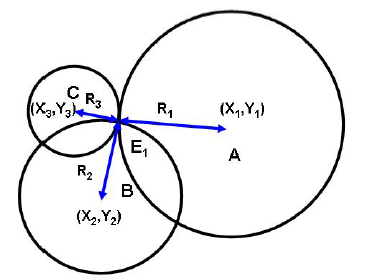
\includegraphics[scale=1]{graphics/triangulation.png}
		\caption{Triangulation\cite{Triangulation}}
		\label{fig:triangulation}
	\end{center}
\end{figure}

\subsubsection*{Angle of Arrival}
This category consists of approaches where the angle of the received signal is measured. The angle can be obtained by either having several antennas or being able to rotate a single antenna to find the direction at which the RSSI is strongest. With multiple angles of arrival it is possible to calculate a position based on the intersection of the euclidean vectors going through the antennas.

\subsubsection*{Location Patterning}
The location patterning category sets out to measure the connectivity patterns for a set of locations. The most common approach for this category is called WI-FI Fingerprinting. This method has an intial calibration phase, where the RSSI pattern for each point of interest is measured and stored in the system. When the signal strength from a device is received, it is then compared to the previously measured RSSI patterns. The point of interest with the most similar pattern is determined to be the position of the device. This means that a system using fingerprinting can not determine the exact position of a device, but rather calculates a probability that the device is located at a given point of interest\cite{fingerprint1}.

\subsection{Evaluation dimensions}
When evaluating indoor location services there are three dimensions that we can evaluate quality on: location precision, refresh rate and system latency. Location precision tells us about the location precision that the system affords. Refresh rate is the rate at which the location is updated, and as such how closely the most recent data is related to real-time data. System latency is a dimension describing the time it takes to perform the positioning calculations\cite{dimensions}. Depending on the usage of the system, the dimensions can be valued using a scale of importance, such as "High", "Medium" and "Low". Alternatively we can chose to look for systems with one or more dimensions below a set value. For instance, we have a desire to find a system with a location precision lower than the average precision for GPS which in 2014 was set to have four meters of inaccuracy \cite{gps_report}. 
\ofx{Should be cite buy cant compile when i change it}

The three dimensions are in no way constant for a system. For most systems, the hardware has a large influence on the dimensions. For instance, location precision for Triangulation is severely diminished if the environment lacks access points. Refresh rate depends on how often mobile devices communicate with the network and system latency can be impacted by a large amount of noise on the WI-FI channels. \Cref{tab:evaluating_approaches} shows the influences for the four tracking approach categories for each evaluation dimension. The system latency of a system entirely depends on the software, hardware and communication protocols used.

\begin{table}[]
\centering
\begin{tabular}{|l|p{4cm}|p{4cm}|p{3.5cm}|}
\hline
                    & Location Precision                 & Refresh Rate             & System Latency    \\ \hline
Cell of Origin      & Within cells                       & On checkpoint register   & Depends on system \\ \hline
Distance            & Depends on amount of access points & When device communicates & Depends on system \\ \hline
Angle of Arrival    & Depends on amount of antennas      & When device communicates & Depends on system \\ \hline
Location Patterning & Depends on calibration phase       & When device communicates & Depends on system \\ \hline
\end{tabular}
\caption{Evaluation dimension in relation to the four tracking approaches}
\label{tab:evaluating_approaches}
\end{table}

\subsection{Technologies}
In this section we examine some systems using different tracking approaches that aStep can use to integrate indoor positioning.

Zonith Indoor Positioning System is a system that uses the cell of origin approach. As mentioned in \cref{sec:tracking_approach}, this technique requires auxiliary hardware. Zonith offers Bluetooth Beacons, which serve as checkpoint nodes, and allow for any device with Bluetooth to be discovered and tracked\cite{zonith}.  Because of the nature of the approach we expect the location precision is excellent at the moment the device is registered, and the quality of the data decays as it ages. However, the most recent registration of a device is an approximation of its location, at best it tells us what room the device is in.

Redpin is an open source indoor positioning system that uses location patterning. The system requires a calibration phase, where the connectivity fingerprint of different key locations is measured. A users location is calculated on request, and, with enough fingerprint meaasurements, the system will be able to provide the user with at least room-level accuracy\cite{redpin}. Location precision is as such dependent on the calibration phase, but is expected to be better than a cell of origin approach. 

Google have also developed their own positioning system. They have made indoor navigation and tracking possible trough their Indoor Maps project \cite{IPSoverGPS}, which lets users map a building by uploading a floor plan of said building. After the floor plan has been accepted, the system will request information about the location of the WI-FI access points in the building\cite{googleindoormaps}. A user can then see their own location on Google maps at any time. Google have been very secretive in regards to what tracking approach they use, as such it is difficult to evaluate the technology.

Cisco have developed a location-aware wireless network system, Cisco Mobility Services Engine (MSE), which utilises WI-FI triangulation\cite{CiscoTri}. MSE makes it possible for Cisco to track the location of up to 25000 network devices at once, regardless of whether the devices are connected to the network. Using the RSSI data from the access points, the Cisco controller calculates distance and compares time of arrival to perform a triangulation and obtain a position\cite{ciscoMSE}.
The building is modelled by the use of an outline of the floor plan. The image is converted to a coordinate system that is placed on top of the model, which is then supplied with the positions of the static access points in the building. With this information it is possible to get the relative position of any device in relation to the origin of the coordinate system. It is these relative positions that are used to track wireless devices.
Cisco claim to have a location precision of less than a meter, refresh rate of 10-120 updates per minute and a system latency of 2-4 seconds\cite{dimensions}. 

\subsection{Choice of Technology}\label{subsec:cisco}
We have presented four technologies using different tracking approaches. We impose two requirements for the technology. First, we largely prefer a system with an accurate location precision. In practice this means being able to position people within rooms, as indoor environments can differ greatly in room size. For instance, an airport is difficult to partition into rooms, as it normally exhibits very open spaces. Secondly, we wish to harvest as much data, in terms of positions, as possible. This allows for predictions on crowd movements, path-finding to circumvent crowded areas and analysing typical movement in a building. 

Our first requirement excludes the Zonith Indoor Positioning System. To accommodate the second requirement, we examine the obtainable data from the systems. Redpin affords the possibility to request the position of a single device. Given that it is open source, it will be possible to alter the system in such a way that all devices on the network is provided. Google Indoor Maps only allows requesting a single user. Cisco MSE has the functionality to provide a list of devices registered along with their most recent position.

There are several arguments pointing towards Cisco MSE rather than Redpin. First and foremost, Cisco MSE is in comparison a lot more convenient, as it already affords the desired functionality and requires substantially less set-up time. Secondly, the amount of documentation for Cisco MSE far outweighs what little documentation there is for Redpin. Cisco MSE is a commercial system, and is therefore updated regularly. As of 7/3/2016, Redpin had its most recent update in May 2013. As a consequence of these arguments we chose to integrate Cisco MSE as the indoor positioning system for aStep.

Aalborg University uses the standard version of Cisco MSE to position devices on their network. We plan on using the data available from this system as dummy data for the aStep project.
\section{Permission} \label{sec:permission}
By using MSE it is possible to acquire and store peoples unique MAC address and use this to track them. It is illegal to do so without the individuals acceptance and it is as such necessary to accommodate this regulation when designing the system \cite{TrafficIlligal}.
There have been several trials in Denmark as a consequence of this regulation. A Traffic system has recorded passerbys by registrating the WI-FI signal emitted from their smart phones. This was done with sensors registrating the unique MAC address, which was then hashed and re-hashed in the sensors before being stored. Despite the attempt at obfuscating the users \cite{TrafficIlligal}, it is illegal according to the \textit{Directive on privacy and electronic communications} article 5(3) \cite{CookieDirective} which can be seen in the following quote,

\begin{quote}
\textit{'Member States shall ensure that the use of electronic communications networks to store information or to gain access to information stored in the terminal equipment of a subscriber or user is only allowed on condition that the subscriber or user concerned is provided with clear and comprehensive information...'}
\end{quote}

However, the Danish Business Authority's conclusion was that the system did not fit in \textit{Directive on privacy and electronic communications} due to the end user being unidentifiable \cite{TrafficOK} as described by article 3(1) \cite{CookieDirective}. No sanction was inflicted for this case, however, this illustrates the necessity to obfuscate personal sensitive information.

%http://eur-lex.europa.eu/legal-content/DA/TXT/PDF/?uri=CELEX:31995L0046&from=da
To ensure no such debates are raised in relation to this project, it will be necessary to differ between those who have given their permission to store person sensitive data and those who have not. By differentiating between the two it will be possible to obfuscate and remove personal data, such as MAC addresses, for individuals who has not given their acceptance.

We will use the term person sensitive data when referring to data that can be used to identify a person. 
\section{Using Cisco}\label{sec:cisco_usage}
The Cisco localisation and positioning system is already in use at Aalborg University. To be able to use the information from the system, we had a meeting with the administrator, during which he raised concerns for privacy, because of the legality of storing person sensitive data, as mentioned in \cref{sec:permission}. Furthermore he wishes to be able to provide the location data to future student projects with ease. To accommodate this, it has been asked of us to build and deploy an intermediate service with the goal of obfuscating sensitive personal data, such as MAC-addresses and user names. This service is intended to duplicate the functionality of the Cisco MSE RESTful API, such that the service acts as a transparent proxy. This is achieved by creating an intermediate RESTful service, that simply redirects requests and processes the response before sending it back to the initial requester, as illustrated on \cref{fig:cisco_usage}.

\begin{figure}[ht]
	\begin{center}
	\includegraphics[scale=0.9]{graphics/cisco_usage.png}
	\caption{Cisco usage}
	\label{fig:cisco_usage}
	\end{center} 
\end{figure}

A RESTful service typically communicates using the HTTP or HTTPS protocols, and functions by receiving requests for specific data resources, called Uniform Resource Identifiers (URIs) to which it responds by sending the requested data. As an example we can send a HTTPS GET request to 64.103.26.61, which is a Cisco MSE test server, with the URI "/api/contextaware/v1/location/clients" and, given that we supply the correct user name and password, receive a string of data corresponding to the type of request \cite{restful_oracle}.

To create a transparent RESTful service that duplicates the functionality of the Cisco RESTful API, we need to make use of the same URIs as the Cisco API\cite{cisco_mse_api}. This is done with the use of the Jersey Java library, which affords the possibility of creating a HTTP server and specifying what URIs are available for a client to request.

\begin{lstlisting}[caption={Adding a URI},label={lst:context_code},language=inc_Java]
server.createContext("/api/contextaware/v1/location/clients", httpExchange -> {
            if (VerifyConnection(httpExchange) == false){
                return;
            }

            String response = CollectAllClients(username, password, ciscoIp);
            httpExchange.sendResponseHeaders(200, response.length());
            OutputStream os = httpExchange.getResponseBody();
            os.write(response.getBytes(Charset.forName("UTF-8")));
            os.close();
        });
\end{lstlisting}
The code example shown on \cref{lst:context_code} shows an example of how to specify a URI. The createContext() method on line 1 takes two parameters: a string for the URI and an anonymous function implementing an interface. The anonymous function taking up the rest of the example dictates what actions are performed once a connection is established. In this case some verification is performed immediately after the function call, to authenticate the user. A response is generated based on the URI; on line 4 we retrieve all clients from Cisco using the ColletAllClients() function, which also performs the task of obfuscating necessary information. The list of clients is then written though an OutputStream to the requester, as seen on lines 8 and 9. The anonymous function terminates as the OutputStream is closed, which also serves as a termination of the HTTP connection. 

In order to accommodate the privacy concern, we implement some simple methods to obfuscate MAC-address and user name, one of which can be seen in \cref{lst:obfuscating_mac}. It might be the case that users allow for us to store their personal information, and as such we will have to make a check to see if this has been allowed. To store this information we use a TreeSet, which guarantees $log(n)$ time cost for adding, deleting and searching \cite{treeset}. On line 2 we obtain the MAC-address of the user, which is used on line 3 to perform a search in the TreeSet. If search returns empty we obfuscate the MAC-address, as seen on line 4. This is done in a similar way for the user name.

\begin{lstlisting}[caption={Obfuscating mac-address},label={lst:obfuscating_mac},language=inc_Java]
Private static Client ObfuscateMacAddress(Client singleClient) {
    String oldMacAddress = singleClient.getWirelessClientLocation().getMacAddress();
    if (!watchList.contains(oldMacAddress)) {
        singleClient.getWirelessClientLocation().setMacAddress(obfuscatedAddress);
    }
    return singleClient;
}
\end{lstlisting}

\subsection{System hierarchy}
With this code it is possible to create an intermediate service for the Cisco MSE RESTful service, that intercepts the response and obfuscates certain information. To use this service, a client needs to know the IP address and a login for the intermediate service. To automate the requests and create a flow of data from the Cisco systems to the aStep database, we will have to build and implement a client that fetches data at an interval. The scope of the project is beyond Aalborg University, and as such we want to integrate more than a single Cisco MSE system. 

\begin{figure}[ht]
	\begin{center}
	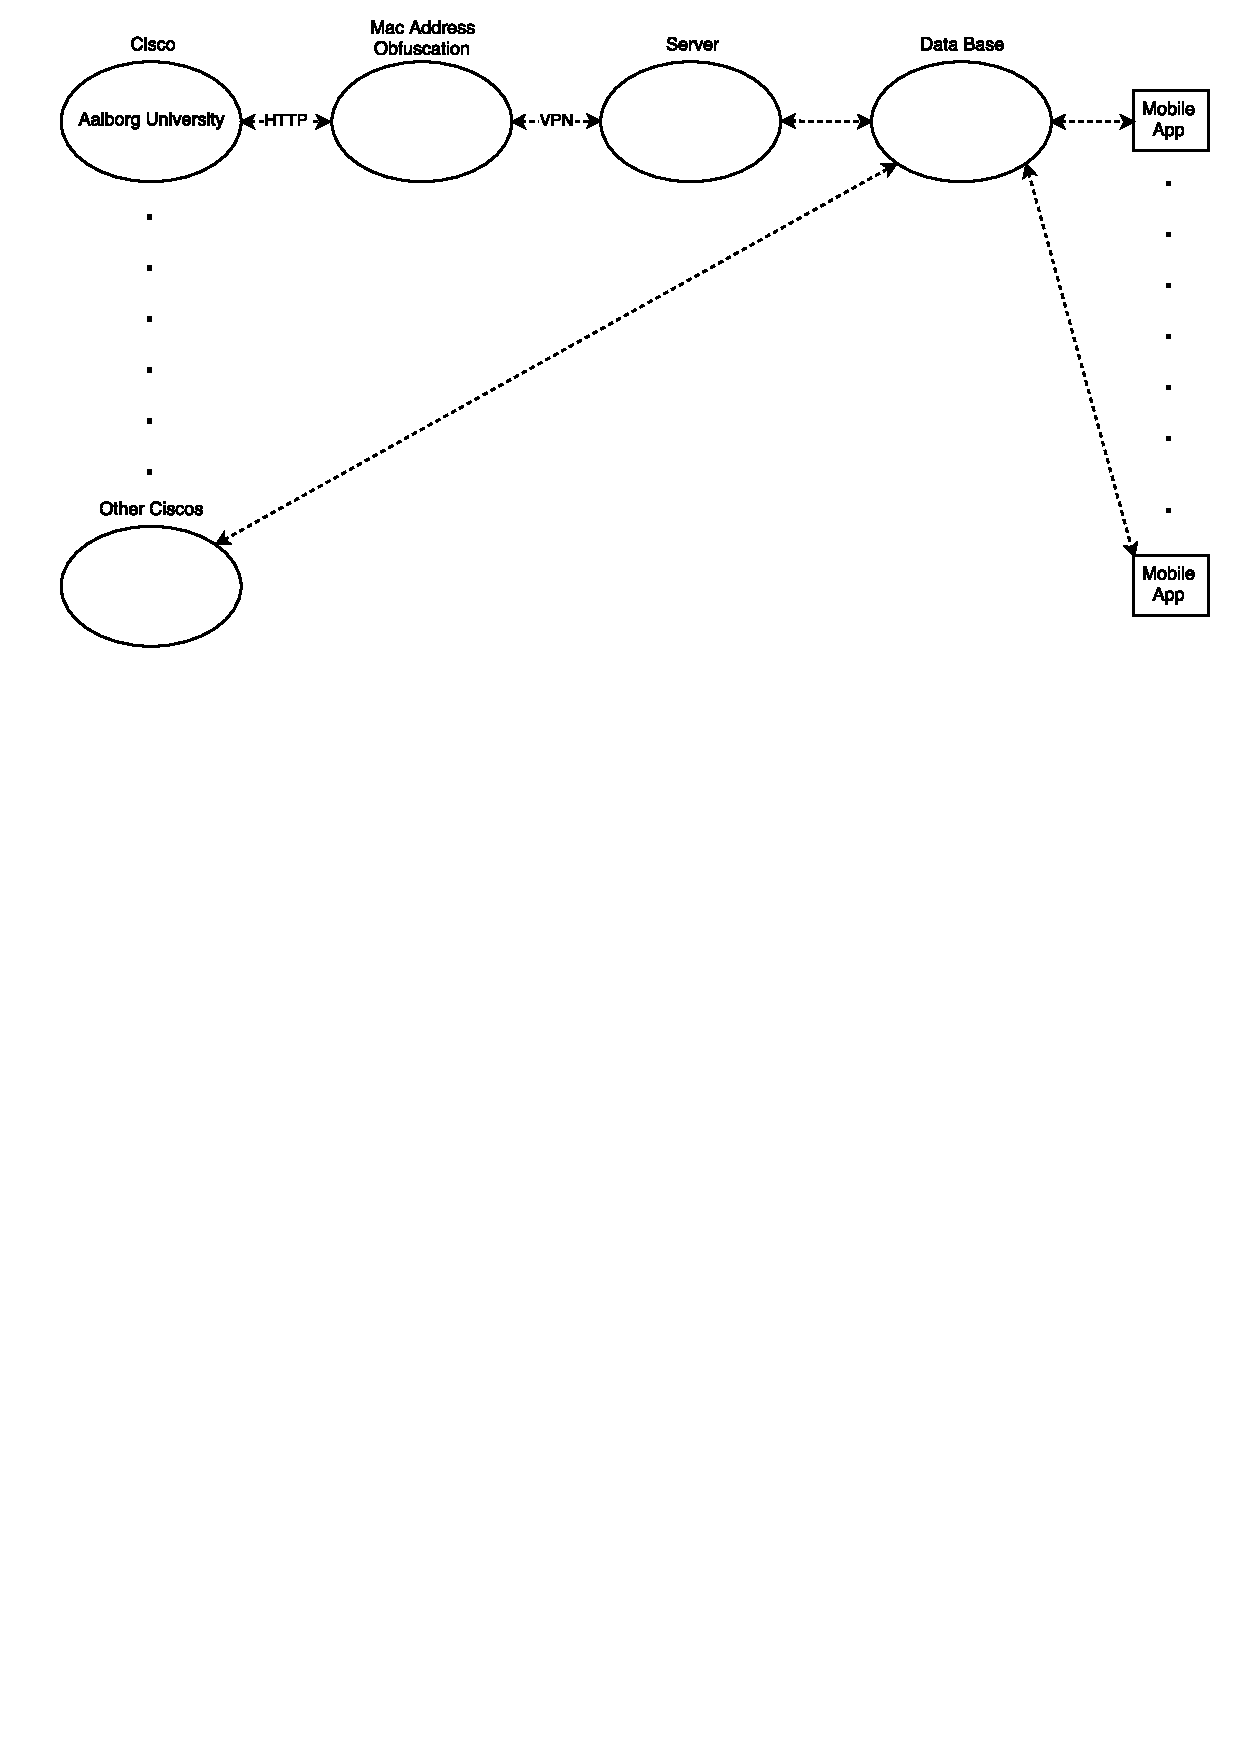
\includegraphics[scale=0.5]{graphics/ciscoSmall.pdf}
	\caption{Cisco systems}
	\label{fig:cisco_systems}
	\end{center} 
\end{figure}
\Cref{fig:cisco_systems} shows how the information flow is intended. The client connecting to the Cisco services can function as a server that requests data from all Cisco services that we have access to. Alternatively, a server can be implemented for each Cisco service. However, this solution has several downsides. First, it means corporations supplying the aStep project with information will have to have hardware running the server, which requires maintenance. Second, this solution is not scalable. The server running the aStep database will potentially be overloaded, as it has to handle each individual Cisco system sending information. As more Cisco systems are added, there will be less time to process received data. An alternative approach is to have the aStep database server request data, however, with an increase in connected Cisco systems, the interval at which we receive new information from a given system also increases. The optimal solution to this issue is to create a hierarchy of servers, such that the database server only receives data from a constant amount of intermediate servers, each of which also receive information from an amount of sources. During the start up of the aStep project we have access to a single Cisco MSE system, and as such we will not focus on building this hierarchy. However, as the project grows and additional Cisco systems are integrated, it will eventually become a necessity.  

\section{Sprint Evaluation}
To conclude on the first sprint, we have explored different methods and technologies to perform indoor positioning. Furthermore we have described certain issues related to person sensitive data, and finally we developed an initial design of a RESTful service to operate as an intermediate service for MSE. 

As such the goals for the first sprint have been fulfilled.